% !TeX program = xelatex
\documentclass[11pt,a4paper]{article}
\usepackage[margin=25mm]{geometry}
\usepackage{amsmath,booktabs,graphicx,float}
\usepackage{tikz}
\usetikzlibrary{arrows.meta}
\graphicspath{{Figures/}{docs/RMFS/Papers/2026_11_MobileRobotTrafficControl_EnergyAndMakespan/Figures/}}
\usepackage[hidelinks]{hyperref}

\title{Mobile Robot Traffic Control at Admissible Stopping Points\protect\\
to Minimize Energy Consumption and Makespan}
\author{Moon Ho Hwang}
\date{November 23, 2026}

\begin{document}
\maketitle

\begin{abstract}
We study traffic control for mobile robots following approved paths with two
objectives: reducing fleet battery energy consumption and makespan. Swept
regions identify spatial interference and determine which parts of a route
can be approved together. A Discrete Event System Specification (DEVS)
model executes the resulting traffic decisions with continuous motion
profiles and event-based clearance reports. We compare requiring a stop
before further movement with allowing rolling passage. We separately vary whether selected intersections
may serve as temporary stopping points. Preliminary simulations show two
effects of parking inside an intersection: it can delay crossing traffic,
and it can free an upstream intersection and let a queue pass. We estimate
battery energy from executed motion histories under
explicit mass, power, and drive assumptions. In both small layouts,
allowing rolling passage reduces estimated energy and makespan relative to
requiring a stop under the same policy for stopping in the intersection. The preferred stopping policy depends
on the layout. In a warehouse simulation with 30 robots and 100 orders,
allowing both rolling passage and intersection stopping yields the lowest
makespan and estimated energy among the four policies tested.
\end{abstract}

\section{Related work}

\subsection{Sweep-based coordination and execution}
O'Donnell and Lozano-P\'erez~\cite{odonnell1989} used intersections of segment
sweeps to construct collision-free, deadlock-free executions of two prescribed
manipulator paths. Their coordination diagram represents one or both robots
advancing and handles endpoint blocking. This is the geometric precedent for
our sweep checks and admissible waits. Our comparison concerns the timed
execution of mobile-robot traffic, including whether a shared intersection is
available as temporary storage and how that choice affects fleet energy and
makespan.

H\"onig et al.~\cite{hoenig2019} use an Action Dependency Graph to preserve
precedence from a warehouse multi-agent pathfinding plan. Their controller
can execute consecutive forward actions continuously and overlap replanning
with execution. Warehouse simulations and a mixed-reality robot experiment
demonstrate the execution framework. SOCS shares the goal of avoiding
unnecessary stops. Its experiment varies the permitted stopping endpoints and
the timing of admission independently, and extends a movement using a
pre-braking request or a verified clearance report.

\subsection{Energy-aware intersection control and downstream blocking}
Malikopoulos et al.~\cite{malikopoulos2018} determine intersection timing
under safety and throughput constraints, then optimize the acceleration of
each connected vehicle. Their simulation reports reduced fuel use and shorter
travel time as vehicles preserve momentum through the intersection. Their
formulation optimizes a continuous control input for the planned crossing.
SOCS instead compares discrete movement permissions and profile extensions
on prescribed paths, with actual footprint clearance as the release event.

Pan et al.~\cite{pan2021} optimize speed profiles for battery-electric
vehicles under a fixed FIFO crossing order using decentralized model predictive
control. Their numerical comparison with centralized optimization shows the
energy--travel-time trade-off for different prediction horizons. This is a
close comparison for our matched-order experiments. Their decision variable
is the predicted speed trajectory. Our current experiments vary whether a
robot may stop inside a shared region and whether permission can extend an
already executing profile.

Verbeke et al.~\cite{verbeke2008} model an intersection as interacting
queues and use Monte Carlo simulation to study stochastic arrivals and service.
Their model accounts for vehicles stranded in the conflict area by downstream
spillback. In saturated and oversaturated cases, accounting for these
interactions yields lower estimated capacity and higher delay than the models
they compare against. SOCS examines individual robot footprints and tests
both effects on a fixed layout: occupying one intersection can block its
cross traffic while releasing a queue at the adjacent upstream intersection.

\subsection{Fleet energy optimization and measurement}
Riazi et al.~\cite{riazi2021} use optimization to improve scheduling and
routing for an industrial AGV system, including adjustment of cruise speed.
Using plant data, they report about 38\% lower energy consumption relative to
their existing controller, with better makespan, lateness, and tardiness.
Their result involves changes in travel distance and cruise speed. Our matched
fixed-route comparisons isolate changes in when and where robots wait and
resume motion.

Ma\l{}opolski et al.~\cite{malopolski2025} compare Chain of Reservations
and Structural On-line Control Policy with shortest- and fastest-path
selection on a square-topology multi-AGV system. They parameterize simulation
with electrical measurements from a real AGV and construct Pareto fronts for
total energy and makespan across fleet sizes. This is a direct precedent for
evaluating fleet traffic rules using both outcomes. SOCS studies a different
decision: whether to reserve an admissible intermediate stop through a
geometric sweep check and whether verified release justifies continuing
without completing the planned stop.

Mei\ss ner and Massalski~\cite{meissner2020} measure battery voltage and
current on a rack-lifting Robotnik RB1 Base and model translation, rotation,
and lift/lower operation. Measured translation and rotation energy increase
with payload in their tests. Some braking runs exhibit negative electrical
power. Their measured movement modules inform the power terms required for
our motion histories. SOCS uses those histories to compare traffic decisions;
its own battery parameters still require calibration.

Sperling and Furmans~\cite{sperling2024} integrate state-dependent power
in an AGV energy model validated against measurements from two industrial
mobile robots over 461 operating hours. Their study demonstrates a way to
estimate energy with speed, load and utilization represented explicitly.
Our implementation integrates over DEVS motion intervals and profile
changes. A state model that groups all driving into one value would
require further calibration before it could quantify the benefit of removing
individual braking and restart cycles.

\begin{table}[htbp]
\centering\small
\caption{Potential contributions relative to the reviewed literature and
the evidence needed to support each claim.}
\label{tab:conditional-contributions}
\setlength{\tabcolsep}{4pt}
\begin{tabular}{@{}p{.15\linewidth}p{.24\linewidth}p{.25\linewidth}p{.30\linewidth}@{}}
\toprule
Decision & Results in prior work & Potential contribution of SOCS & Success condition \\
\midrule
Geometric execution & Segment sweeps support feasible path coordination;
action dependencies support continuous execution of forward moves
\cite{odonnell1989,hoenig2019}. & Isolate the effects of admissible command
endpoints and event-triggered continuation. & Complete the same routes under
matched safety constraints. Report intermediate stops and makespan for
each cell of the $2\times2$ comparison. \\[3pt]
Intersection approach & Optimal control and predictive control shape vehicle
speed and report travel-time and energy or fuel benefits
\cite{malikopoulos2018,pan2021}. & Measure the benefit of pre-braking requests
and verified release with fixed routes and crossing orders. & Show fewer
stops and lower net battery energy than requiring a stop under the same
motion and occupancy constraints. Compare directly with a predictive
baseline before claiming an advantage over predictive control. \\[3pt]
Intersection storage & Queue spillback simulations capture capacity loss
and cross-traffic delays from blocked intersections \cite{verbeke2008}. &
Identify when using an intersection as a buffer releases upstream traffic
at the cost of delaying cross traffic. & Reproduce cases with opposite
outcomes. Measure upstream queue clearance, cross-traffic delay, and
makespan. For a conditional policy, compare with both fixed policies on
additional congestion cases. \\[3pt]
Fleet objectives & Industrial AGV studies evaluate energy and completion
time under routing, scheduling, speed or deadlock-policy changes
\cite{riazi2021,malopolski2025}. & Evaluate energy and makespan trade-offs
for stopping and admission policies on identical routes and workloads. &
For a joint improvement, show lower energy at the same or lower makespan,
or lower makespan at the same or lower energy. Report the trade-off when
one objective improves and the other worsens. \\[3pt]
Energy evaluation & AGV measurements support physical and state-dependent
power models \cite{meissner2020,sperling2024}. & Attribute differences in net
battery energy to realized waits, braking and restart cycles. & Check Wh
against measured power traces or disclose calibration uncertainty. Verify
that identical physical histories and observation horizons give the same
energy across headless runs and animation intervals. \\
\bottomrule
\end{tabular}
\end{table}

\section{Control problem}
Each robot has a fixed path and a set of admissible stopping points. At an
admissible point it may wait or continue to a subsequent point. A traffic
policy selects the points at which waiting is permitted and governs when
the next part of the path is approved. An intersection may act as a
temporary buffer if a stationary robot there clears an upstream constraint.
Its occupancy may meanwhile block traffic on the crossing route.

For a common start time of zero, let $C_i$ denote the time at which robot $i$
completes its assigned path, and let $E_i$ be its net battery energy over a
specified observation horizon. The objectives are
\[
 C_{\max}=\max_i C_i,\qquad E_{\mathrm{fleet}}=\sum_i E_i.
\]
Equation~\eqref{eq:robot-energy} in Section~\ref{sec:energy-model} gives the calculation of $E_i$.
We report both objectives for each policy. The energy estimates apply to the
assumed power model and the executed profiles.

\section{Swept paths and DEVS execution}
\subsection{Swept regions and clearance}
For robot $i$ and a path interval $[a,b]$, the swept region is
$S_i[a,b]=\bigcup_{s\in[a,b]} F_i(s)$, where $F_i(s)$ is the footprint
placed along the path at progress $s$. An interval with $a=b$
represents a stationary footprint. For the axis-aligned translations
used here, the sweep is the union of the rectangular sweeps of the
individual segments. Intersecting sweeps indicate potential spatial
interference between motions.

This geometric use of segment sweeps follows O'Donnell and Lozano-P\'erez
\cite{odonnell1989}. The companion technical report~\cite{hwang2026sweep}
develops subpath sweeps, tuple paths, and residual interference for
fixed-path mobile robots. In the present controller, an arrival or
clearance report advances the released progress. Admission checks
compare a candidate movement with the unpassed portions of approved
sweeps, stationary footprints, and required precedence. A clearance
report can therefore release part of a sweep before the robot reaches
the endpoint of its current command.

\subsection{Remaining path and remaining movement approval}
\label{sec:remaining-movement-approval}
Normalize progress along each registered work leg to $[0,1]$, with $1$
denoting the task destination. Let $p_r$ be the released progress recorded
by the roadmap and $p_a$ the endpoint of the current movement approval.
During an active approval, $p_r\le p_a\le 1$. The remaining path sweep is
$S_i[p_r,1]$, and the remaining approved sweep is $S_i[p_r,p_a]$.
An extension from $p_a$ to $q$ proposes the sweep $S_i[p_a,q]$.
Admission compares the proposed sweep with other robots' stationary
footprints and remaining approved sweeps, and respects the sweeps of
required predecessor movements.

Figure~\ref{fig:remaining-approval} shows how the three sweep intervals
relate along one registered path.

\begin{figure}[H]
\centering
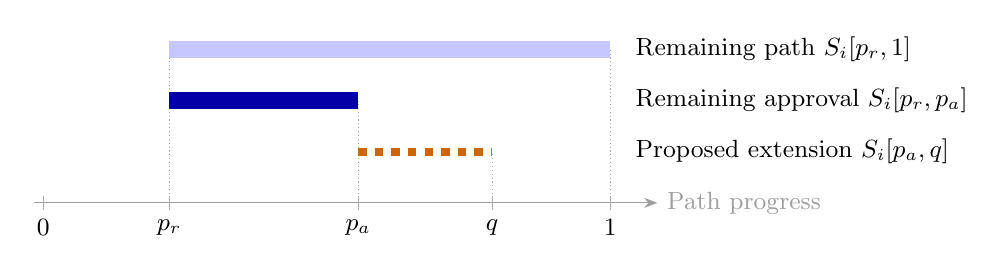
\begin{tikzpicture}[x=1cm,y=.65cm,>=Stealth,
                    every node/.style={font=\small}]
  \draw[->,gray!75] (-.12,0)--(7.8,0) node[right] {Path progress};
  \foreach \x/\labeltext in {0/0,1.6/{p_r},4.0/{p_a},5.7/q,7.2/1}{
    \draw[gray!65] (\x,-.13)--(\x,.13);
    \node[below] at (\x,-.14) {$\labeltext$};
  }
  \foreach \x/\top in {1.6/3,4/2,5.7/1,7.2/3}
    \draw[gray!65,densely dotted] (\x,.17)--(\x,\top);
  \draw[line width=6pt,blue!22] (1.6,3)--(7.2,3);
  \draw[line width=6pt,blue!65!black] (1.6,2)--(4,2);
  \draw[line width=3pt,orange!80!black,dashed] (4,1)--(5.7,1);
  \node[right] at (7.4,3) {Remaining path $S_i[p_r,1]$};
  \node[right] at (7.4,2) {Remaining approval $S_i[p_r,p_a]$};
  \node[right] at (7.4,1) {Proposed extension $S_i[p_a,q]$};
\end{tikzpicture}
\caption{The path intervals underlying the remaining path sweep,
remaining approved sweep, and proposed extension. The bars represent
intervals along the path. Each swept region includes the robot footprint
along its interval.}
\label{fig:remaining-approval}
\end{figure}

Issuing or extending an approval sets or advances $p_a$. A sensor
clearance report advances $p_r$ after the robot's footprint has passed the
reported control point. Merely reaching an intermediate point during
continuous motion does not release it. The controller then recomputes the
sweep from the new release boundary, preserving the portion that can
still be occupied. Arrival at the approved endpoint ends that movement
approval and records the robot's stationary footprint there. Future
movement from that point requires a new approval.

\paragraph{Theorem 1 (Collision-free execution of disjoint approvals).}
Let $S_i$ and $S_j$ be the remaining approved sweeps of two robots at
the time of the check. If $S_i\cap S_j=\emptyset$, the robots cannot
collide while executing those approvals.

\emph{Proof.}
By definition, each sweep is the union of robot footprints over the
poses along its remaining approved motion, including turns and stops.
At any common execution time $t$, the occupied regions therefore satisfy
$B_i(t)\subseteq S_i$ and $B_j(t)\subseteq S_j$. It follows that
$B_i(t)\cap B_j(t)\subseteq S_i\cap S_j=\emptyset$ at every such time.

\paragraph{Theorem 2 (Collision-free approval extension).}
Suppose the current remaining approved sweeps $S_i$ and $S_j$ are
disjoint. Let $E_i$ be the sweep added by extending robot $i$'s approval
endpoint, including any new turn at the join. If $E_i\cap S_j=\emptyset$,
the two robots can execute the updated approvals without collision.

\emph{Proof.}
Robot $i$'s updated remaining approved sweep is $S_i\cup E_i$.
By distributivity,
$(S_i\cup E_i)\cap S_j=(S_i\cap S_j)\cup(E_i\cap S_j)=\emptyset$.
The result follows from Theorem~1.

\subsubsection{Example of a shared path in the same direction}
In Figure~\ref{fig:same-direction-approvals}, red R1 travels from $(0,0)$
to $(6,0)$ and green R3 travels from $(4,0)$ to $(10,0)$. Each robot's
task destination remains fixed. The diamonds mark the current approval
endpoints. The pale bands show the remaining path sweeps, and overlapping
bands of the same color highlight the remaining approved sweeps.

\begin{figure}[H]
\centering
\begin{minipage}{.98\linewidth}
\small
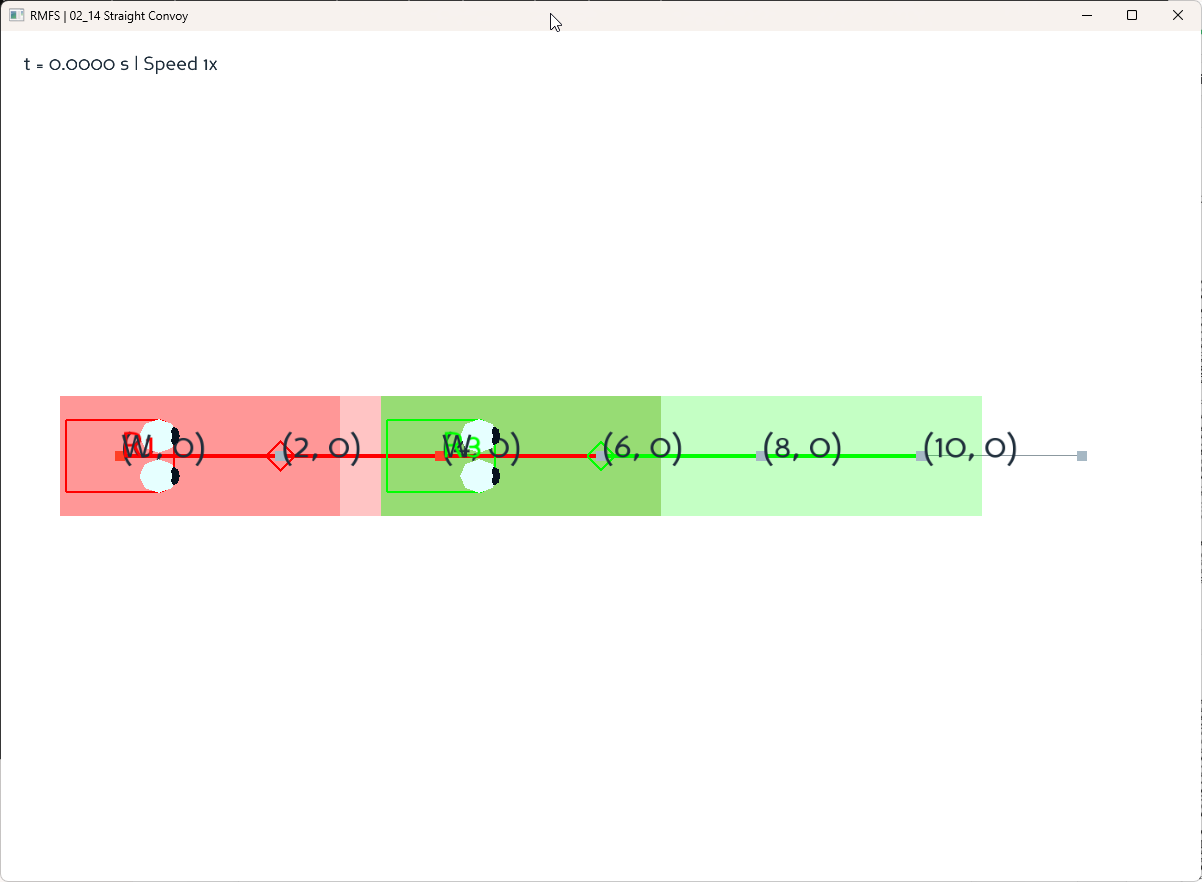
\includegraphics[width=\linewidth,trim=43bp 330bp 95bp 365bp,clip]{shared_path_same_a.png}\par
(a) \textbf{0.0000 s.} R1 is initially approved to $(2,0)$ and R3 to $(6,0)$.
At departure, each pale sweep covers the full path from start to task destination. The point $(6,0)$ is also R1's task destination.\par\smallskip
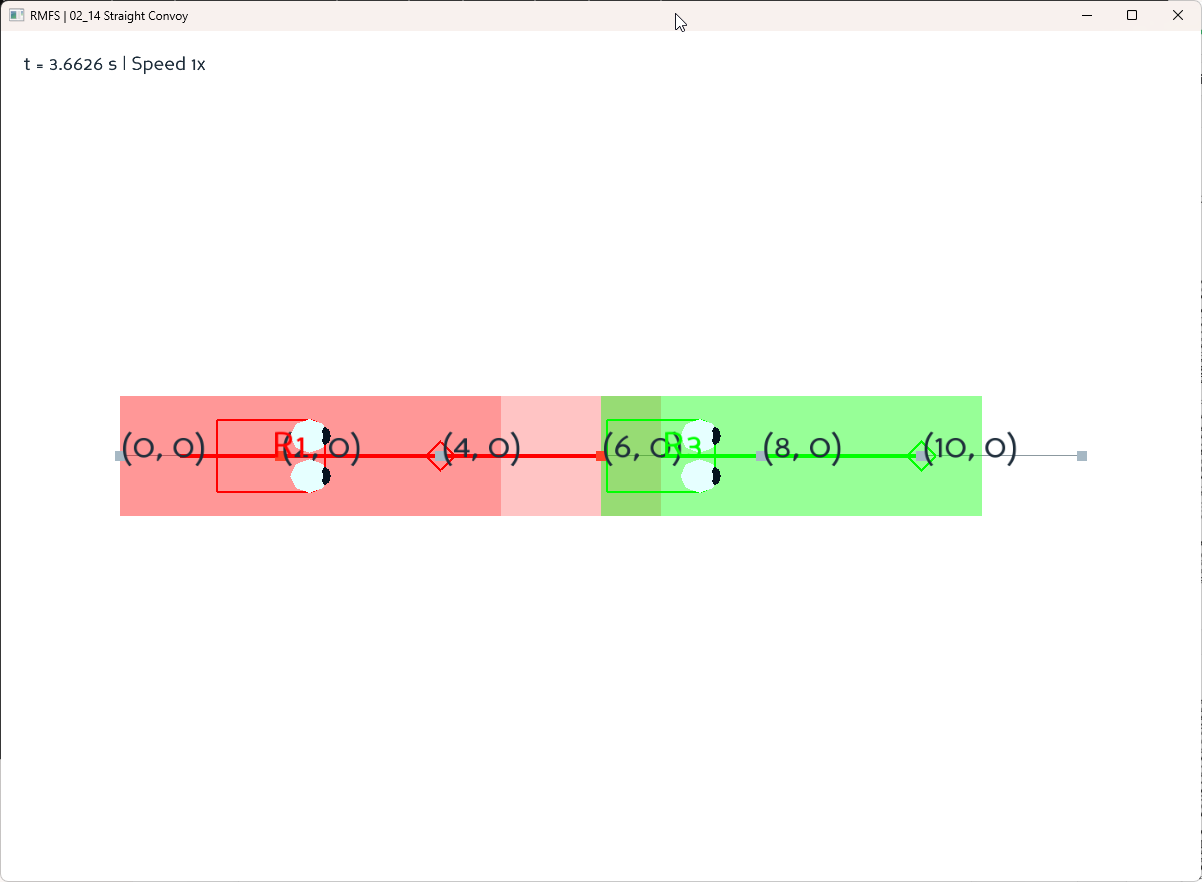
\includegraphics[width=\linewidth,trim=43bp 330bp 95bp 365bp,clip]{shared_path_same_b.png}\par
(b) \textbf{3.6626 s.} R3 is approved to its destination $(10,0)$.
Its clearance report from $(6.75,0)$ lets R1 extend its approval to $(4,0)$.\par\smallskip
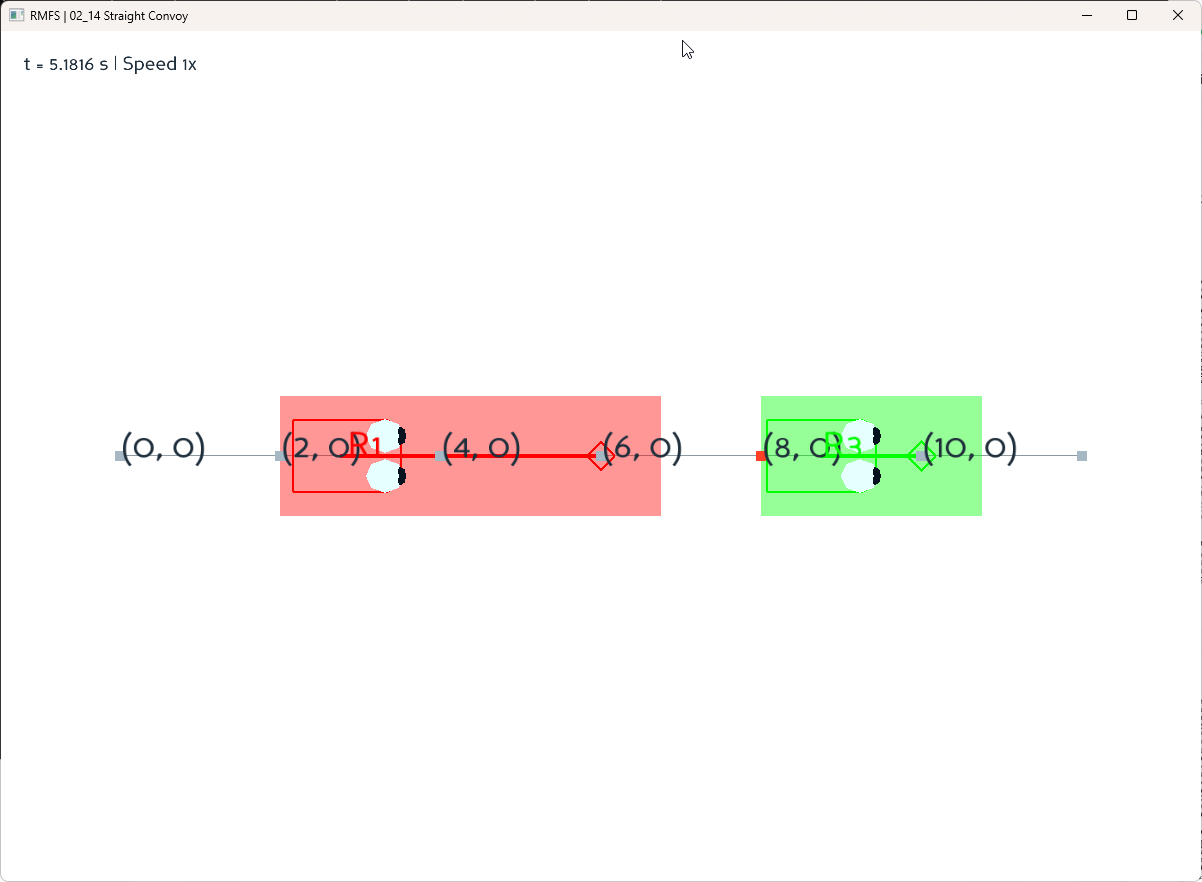
\includegraphics[width=\linewidth,trim=43bp 330bp 95bp 365bp,clip]{shared_path_same_c.png}\par
(c) \textbf{5.1816 s.} R3 reports clearance from $(8.75,0)$.
R1's approval extends to its destination $(6,0)$ while R1 is still moving.\par\smallskip
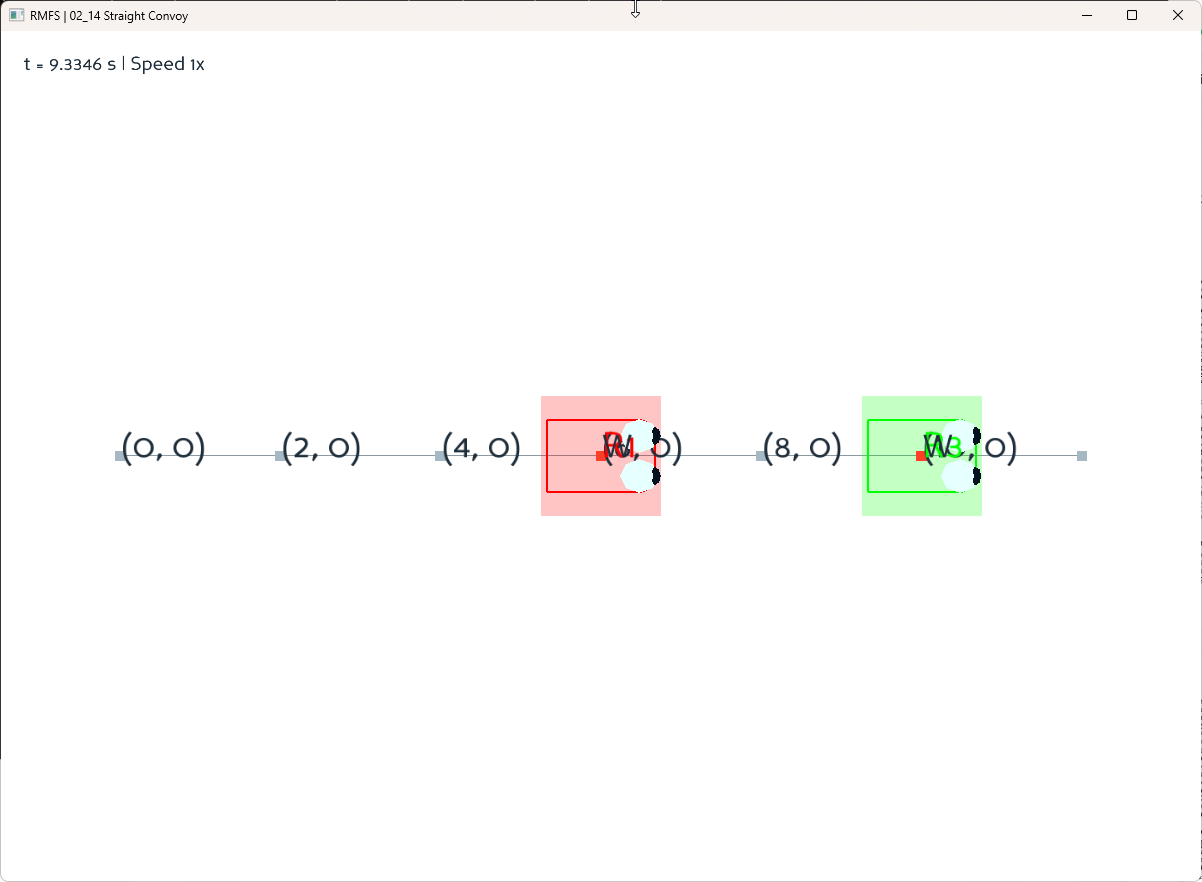
\includegraphics[width=\linewidth,trim=43bp 330bp 95bp 365bp,clip]{shared_path_same_d.png}\par
(d) \textbf{9.3346 s.} R1 has reached $(6,0)$ and R3 is already at $(10,0)$.
The approvals have ended and both robots retain their stationary footprints.
\end{minipage}
\caption{Same-direction travel on an overlapping path. R1 continues
without an intermediate stop as clearance reports from R3 extend its approval.}
\label{fig:same-direction-approvals}
\end{figure}

\clearpage
\subsubsection{Example of alternating clearance on paths with turns}
In Figure~\ref{fig:alternating-approvals}, red R1 travels from $(0,1)$ to
$(3,3)$ and green R2 from $(2,3)$ to $(0,0)$. Each robot starts on a
point the other needs later. The initial approvals span the first turns
and let both robots move away from these points. Coordinates are grid indices.

\begin{figure}[H]
\centering
\newcommand{\AlternatingPanel}[2]{%
  \begin{minipage}[t]{.48\linewidth}\small
  \centering
  \includegraphics[width=.70\linewidth,trim=225bp 58bp 212bp 90bp,clip]{alternating_approval_#1.png}\par
  \raggedright #2\par
  \end{minipage}%
}
\AlternatingPanel{1}{(a) \textbf{0.0000 s.} R1 is approved through the
turn at $(2,1)$ to $(2,2)$. R2 is approved through $(0,3)$ to $(0,2)$.}\hfill
\AlternatingPanel{2}{(b) \textbf{3.1235 s.} Both robots have advanced
along their first straight runs. The approval endpoints remain unchanged.}\par\smallskip
\AlternatingPanel{3}{(c) \textbf{3.7776 s.} Clearance reports release
the space around the two starts. R2 is now approved to its goal $(0,0)$.
R1's approval extends to $(2,3)$, where it must turn again.}\hfill
\AlternatingPanel{4}{(d) \textbf{14.4939 s.} R1 is at $(2,3)$ and has
received a new approval to $(3,3)$ for the final leg after the turn.
R2 is approaching its goal.}\par\smallskip
\AlternatingPanel{5}{(e) \textbf{20.9112 s.} Both robots are at their
task destinations. The colored regions now show their stationary footprints.}
\caption{Alternating clearance and movement approvals on paths with turns.
Pale shading shows the remaining path sweeps. Darker shading shows
remaining approved sweeps, and diamonds mark active approval endpoints.}
\label{fig:alternating-approvals}
\end{figure}
\subsubsection{Example of a shared path in opposite directions}
In Figure~\ref{fig:opposite-direction-approvals}, red R1 travels from
$(0,-4)$ to $(12,4)$, and green R2 travels from $(12,-4)$ to $(0,4)$.
Their routes share the 12~m aisle between $(0,0)$ and $(12,0)$.
The reference plan gives R1 precedence in the aisle. The approach
approvals let both robots move toward their respective entrances.

\begin{figure}[H]
\centering
\newcommand{\OppositePanel}[2]{%
  \begin{minipage}[t]{.48\linewidth}\small
  \includegraphics[width=\linewidth,trim=105bp 80bp 90bp 105bp,clip]{shared_path_opposite_#1.png}\par
  #2
  \end{minipage}%
}
\OppositePanel{a}{(a) \textbf{0.0000 s.} R1 is approved to $(0,-2)$
and R2 to $(12,-2)$. At departure, each pale sweep covers the full path from start to task destination, and the two sweeps overlap along the aisle.}\hfill
\OppositePanel{b}{(b) \textbf{4.4173 s.} R1 receives approval through
the aisle to $(12,4)$. R2 is at its approach point $(12,-2)$.}\par\medskip
\OppositePanel{c}{(c) \textbf{21.7126 s.} R1 has reached $(12,0)$
and still occupies the right junction. R2 remains at $(12,-2)$.}\hfill
\OppositePanel{d}{(d) \textbf{27.0461 s.} R1 has cleared the conflict on its way to $(12,4)$. R2 is still at $(12,-2)$ and is now approved through the aisle to $(0,4)$.}\par\medskip
\OppositePanel{e}{(e) \textbf{52.5884 s.} R2 arrives at $(0,4)$.
Both movement approvals have ended, leaving the stationary footprints.}
\caption{Opposite-direction travel through a shared aisle. Diamonds
mark active approval endpoints. The overlapping pale sweeps in (a)
show both remaining routes before either robot is approved through the aisle.}
\label{fig:opposite-direction-approvals}
\end{figure}

R2 received its through-aisle approval at 27.0461~s (panel (d)), when the controller
received R1's clearance report from $(12,1.51)$. R1's arrival at the right
junction in panel (c) had not yet cleared the conflict. The later
clearance report allowed R2 to start before R1 reached its destination.


\subsection{Coupled DEVS model}
Figure~\ref{fig:coupled-devs} shows the warehouse model. The
\texttt{OrderGenerator} emits the initial order batch at time zero.
\texttt{RMFSController} dispatches orders and authorizes movements
using its roadmap and traffic manager. Each \texttt{MRobot} executes
motion and rack handling, and its paired \texttt{PSensor} schedules
point-clearance reports from the executed motion plans. The
\texttt{MotionEnergyCollector} records motion, arrival, and load
events during the warehouse energy runs. The three control and
execution models are described in Appendices~\ref{app:rmfs-controller},
\ref{app:mrobot}, and~\ref{app:psensor}.

\begin{figure}[H]
\centering
\setlength{\unitlength}{1pt}
\begin{picture}(430,175)
  \put(0,0){\framebox(430,175){}}
  \put(10,159){\makebox(0,0)[l]{\small\textbf{RMFS coupled DEVS}}}
  \put(12,112){\framebox(112,25){\small\texttt{OrderGenerator}}}
  \put(167,112){\framebox(112,25){\small\texttt{RMFSController}}}
  \put(12,22){\framebox(112,25){\scriptsize\texttt{MotionEnergyCollector}}}
  \put(167,22){\framebox(112,25){\small\texttt{MRobot}$_i$}}
  \put(316,22){\framebox(102,25){\small\texttt{PSensor}$_i$}}
  \put(124,125){\vector(1,0){43}}
  \put(145,134){\makebox(0,0){\scriptsize orders}}
  \put(187,112){\vector(0,-1){65}}
  \put(182,86){\makebox(0,0)[r]{\scriptsize move, orient, extend}}
  \put(182,74){\makebox(0,0)[r]{\scriptsize lift and lower}}
  \put(241,47){\vector(0,1){65}}
  \put(246,86){\makebox(0,0)[l]{\scriptsize arrival, rotation}}
  \put(246,74){\makebox(0,0)[l]{\scriptsize load and passage events}}
  \put(279,34){\vector(1,0){37}}
  \put(298,16){\makebox(0,0){\scriptsize motion plan}}
  \put(367,47){\line(0,1){78}}
  \put(367,125){\vector(-1,0){88}}
  \put(323,134){\makebox(0,0){\scriptsize clearance reports}}
  \put(167,34){\vector(-1,0){43}}
  \put(145,16){\makebox(0,0){\scriptsize recorded events}}
  \put(367,7){\makebox(0,0){\scriptsize $i=1,\ldots,n$ robot--sensor pairs}}
\end{picture}
\caption{Warehouse DEVS components and their principal event couplings.
Passage requests and motion extensions are enabled with rolling passage.
The collector observes events without issuing control commands. When
contact checking is enabled, the coupled model injects collision events,
and sensors relay collision reports to the controller.}
\label{fig:coupled-devs}
\end{figure}

In \emph{Stop required} mode, the robot stops at its currently approved
endpoint before receiving its next movement. In \emph{Rolling passage
allowed} mode, the robot can continue without stopping if a movement
extension is approved in time. We implement reconsideration during motion
with a pre-braking request (Push event) or a verified clearance report
(Pull event). An admissible straight continuation can extend the active
motion profile. The \emph{Stopping in intersection} policy independently determines whether an approved movement can end there.

\section{Experimental evaluation of makespan and energy}
\subsection{Experimental design and energy model}
\label{sec:energy-model}
For each small layout we vary \emph{Rolling passage} and \emph{Stopping in intersection} in a $2\times2$ comparison. The initial configuration and routes stay
fixed within each comparison. Each stopping policy uses a validated reference
execution, which can change the passage order. The blocker departs at 16~s
in the three-robot single-crossing case and at 32~s in the five-robot
two-crossing case. Its release is determined by sensor feedback.

In the small-layout experiments every robot carries a rack. The MiR600 chassis
mass is 240~kg and the rated maximum
payload is 600~kg~\cite{mir600}. We set the rack mass to 300~kg, half that
rating, giving a total moving mass of 540~kg per robot. The manufacturer
specifies maximum accelerations of 0.41~$\mathrm{m/s^2}$ at zero payload and
0.37~$\mathrm{m/s^2}$ at maximum payload, and a maximum speed of
2~$\mathrm{m/s}$~\cite{mir600datasheet}. We use the full-load acceleration
limit for the 300~kg rack. The cited specifications give no separate normal
braking values, so we set each braking magnitude equal to its acceleration
limit as a model assumption. The masses, speed limits, acceleration and
braking values, and power-model parameters are supplied through
\nolinkurl{Data/mir600_energy_inputs.json}. All alternatives use the same
collision envelope. The small-layout routes consist of straight movements.

Table~\ref{tab:motion-profiles} gives the acceleration, cruise, and braking
parameters of the DEVS robot. For a rest-to-rest motion, if the
distance or angle is too short to reach the speed limit, the robot transitions
directly from acceleration to braking. The yaw parameters are simulation
calibration values chosen to give $90^\circ$ turns of 2~s without a rack
and 3~s with a rack. The acceleration, cruise, and braking phases of the
$90^\circ$ turn last 0.390, 1.219, and 0.390~s without a rack, and 0.227,
2.547, and 0.227~s with a rack, respectively.

\begin{table}[H]
\centering
\small
\caption{DEVS motion profiles by load state. Braking is given as a magnitude,
and cruise speed is the upper limit.}
\label{tab:motion-profiles}
\begin{tabular}{@{}llrrrr@{}}
\toprule
Motion & Load & Acceleration & Cruise speed & Braking & $90^\circ$ time \\
\midrule
Straight & Empty & $0.41\,\mathrm{m/s^2}$ & $2.00\,\mathrm{m/s}$ &
  $0.41\,\mathrm{m/s^2}$ & \textemdash \\
Straight & Rack & $0.37\,\mathrm{m/s^2}$ & $2.00\,\mathrm{m/s}$ &
  $0.37\,\mathrm{m/s^2}$ & \textemdash \\
Rotation & Empty & $2.50\,\mathrm{rad/s^2}$ & $0.97586\,\mathrm{rad/s}$ &
  $2.50\,\mathrm{rad/s^2}$ & $2.000\,\mathrm{s}$ \\
Rotation & Rack & $2.50\,\mathrm{rad/s^2}$ & $0.56637\,\mathrm{rad/s}$ &
  $2.50\,\mathrm{rad/s^2}$ & $3.000\,\mathrm{s}$ \\
\bottomrule
\end{tabular}
\end{table}

The eight small-layout cases were rerun with the calibrated yaw profiles.
None executed a rotation, and all reported makespan and energy values
were reproduced to the precision shown. The warehouse runs also used
the calibrated yaw profiles.

Following the physical decomposition of AGV power in~\cite{meissner2020},
we estimate electrical draw on a level floor using
\begin{align}
 P_i(t)&=P_{\mathrm{aux}}+
 \frac{\max\{0,m_i[a_i(t)+c_r g]v_i(t)\}}{\eta},
 \label{eq:robot-power}\\
 E_i&=\frac{1}{3600}\int_0^{C_i}P_i(t)\,dt\quad\text{(Wh)}.
 \label{eq:robot-energy}
\end{align}
We use $P_{\mathrm{aux}}=40$~W, $c_r=0.025$, $g=9.81$~$\mathrm{m/s^2}$, and
$\eta=0.75$. We assume no regenerative recovery. Auxiliary power is charged
from time zero through each robot's own final arrival. This accounts for all
waiting, including the prescribed blocker hold. Post-completion idle time is
outside the observation interval.
On each executed constant-acceleration interval, traction energy is the
constant nonnegative drive force times distance divided by efficiency.
Profile extensions preserve the executed prefix and replace the remaining
intervals. No rendering-frame values enter the integral.

\subsection{Results}

For the two small layouts, each alternative is followed by the executed speed profiles and cumulative
battery energy. The energy plot includes every robot and the fleet sum.
Axes are shared across the four alternatives within each layout. Each robot's
energy stays constant after final arrival.

\newcommand{\ProfilePair}[2]{%
  \begin{minipage}[t]{.49\linewidth}%
  \noindent{\small\textbf{#1}}\par\smallskip
  \begin{center}
    \includegraphics[width=\linewidth]{Profiles/#2_speed.pdf}\par\medskip
    \includegraphics[width=\linewidth]{Profiles/#2_energy.pdf}
  \end{center}%
  \end{minipage}%
}

\subsubsection{One crossing}
\begin{table}[H]
\centering
\small
\caption{One crossing. The initial top view shows the three robots and
their full-path sweeps only. The table reports makespan and estimated fleet battery energy.}
\label{tab:one-crossing-results}
\begin{minipage}[c]{.34\linewidth}
\centering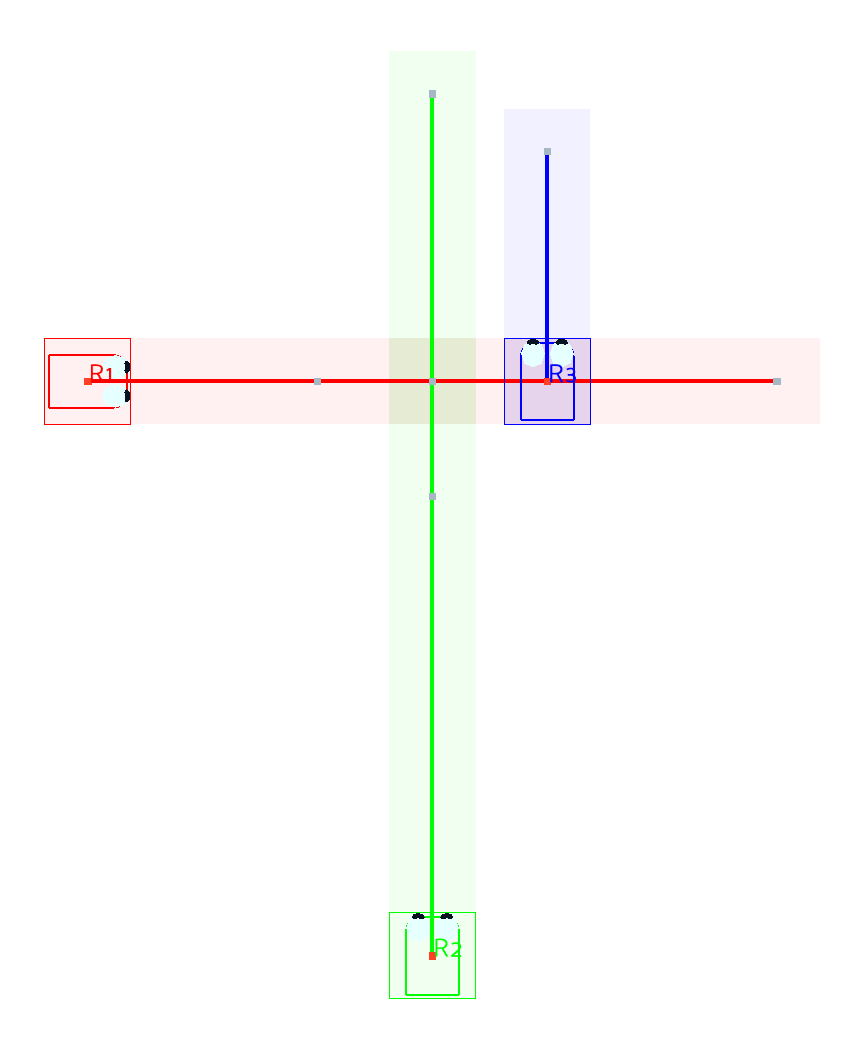
\includegraphics[width=\linewidth]{one_crossing_initial_top.png}
\end{minipage}\hfill
\begin{minipage}[c]{.62\linewidth}
\centering
\begin{tabular}{@{}llrr@{}}
\toprule
\shortstack[l]{Rolling\\passage} & \shortstack[l]{Stopping in\\intersection} & \shortstack[r]{Makespan\\(s)} & \shortstack[r]{Energy\\(Wh)}\\
\midrule
Forbidden & Forbidden & 32.009 & 2.714\\
Allowed & Forbidden & 28.157 & 2.562\\
Forbidden & Allowed   & 33.881 & 2.869\\
Allowed & Allowed   & 30.413 & 2.795\\
\bottomrule
\end{tabular}
\end{minipage}
\end{table}

\clearpage
\noindent\ProfilePair{Rolling passage: Forbidden\newline Stopping in intersection: Forbidden}{one_crossing_stop_first_forbid}\hfill%
\ProfilePair{Rolling passage: Allowed\newline Stopping in intersection: Forbidden}{one_crossing_push_pull_forbid}\par\medskip
\noindent\ProfilePair{Rolling passage: Forbidden\newline Stopping in intersection: Allowed}{one_crossing_stop_first_allow}\hfill%
\ProfilePair{Rolling passage: Allowed\newline Stopping in intersection: Allowed}{one_crossing_push_pull_allow}\par\medskip

\clearpage
\subsubsection{Two crossings}
\begin{table}[H]
\centering
\small
\caption{Two crossings. The initial top view shows five robots, including
the two robots waiting to cross behind R1. The colored overlays show only the full-path sweeps. Energy is the fleet total.}
\label{tab:two-crossings-results}
\begin{minipage}[c]{.34\linewidth}
\centering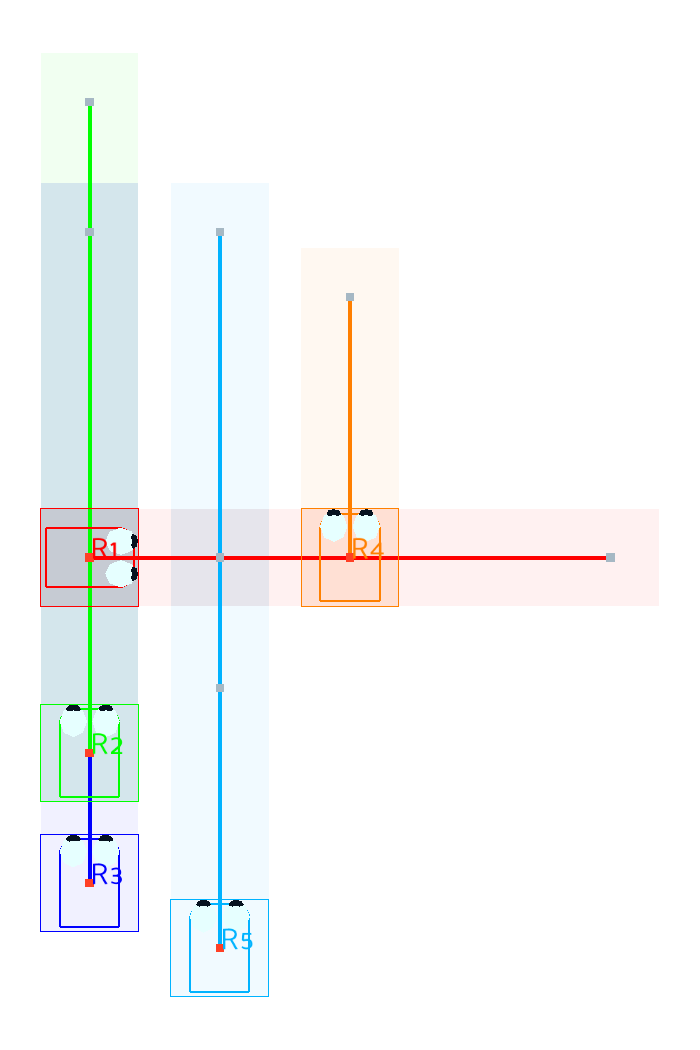
\includegraphics[width=\linewidth]{two_crossings_initial_top.png}
\end{minipage}\hfill
\begin{minipage}[c]{.62\linewidth}
\centering
\begin{tabular}{@{}llrr@{}}
\toprule
\shortstack[l]{Rolling\\passage} & \shortstack[l]{Stopping in\\intersection} & \shortstack[r]{Makespan\\(s)} & \shortstack[r]{Energy\\(Wh)}\\
\midrule
Forbidden & Forbidden & 62.763 & 5.090\\
Allowed & Forbidden & 54.563 & 4.824\\
Forbidden & Allowed   & 49.881 & 4.683\\
Allowed & Allowed   & 46.413 & 4.437\\
\bottomrule
\end{tabular}
\end{minipage}
\end{table}

\clearpage
\noindent\ProfilePair{Rolling passage: Forbidden\newline Stopping in intersection: Forbidden}{two_crossings_stop_first_forbid}\hfill%
\ProfilePair{Rolling passage: Allowed\newline Stopping in intersection: Forbidden}{two_crossings_push_pull_forbid}\par\medskip
\noindent\ProfilePair{Rolling passage: Forbidden\newline Stopping in intersection: Allowed}{two_crossings_stop_first_allow}\hfill%
\ProfilePair{Rolling passage: Allowed\newline Stopping in intersection: Allowed}{two_crossings_push_pull_allow}\par\medskip

\subsubsection{Comparison across layouts}
In the single-crossing layout, the robot that stops in the intersection
blocks the cross route while waiting for its exit. In the two-crossing
layout, using the forward intersection as a buffer frees the rear crossing.
With rolling passage allowed, the last robot in the rear queue clears it at $15.485$~s
with the buffer and $50.177$~s without it. The robot crossing the forward
intersection clears at $42.070$~s with the buffer and $6.562$~s without it.
Forbidding the stop gives the lowest observed makespan and estimated energy
for one crossing (Table~\ref{tab:one-crossing-results}). Allowing the buffer
gives the lowest values for two crossings (Table~\ref{tab:two-crossings-results}).

All eight small-layout runs completed. We replayed the DEVS-only runs with
collision checks at 0.01 and 0.1~s intervals. No contacts were detected in the
replays, and makespan and energy agreed to a relative and absolute tolerance
of $10^{-10}$ in the reported units. These are model estimates. Physical
battery measurements would be needed to calibrate the numerical energy
savings. The experiments compare four policies and do not establish global
optimality. The reproducer is
\begin{quote}\small\ttfamily
python -m examples.RMFS.Tests.run\_crossing\_energy\_comparison --load rack
\end{quote}

\clearpage
\subsubsection{Warehouse order workflow}
We applied the same $2\times2$ policy design to the warehouse workflow with
30 robots, 120 racks, and 10 inbound/outbound workstations. Each run used
100 orders, seed 0, and the same initial layout and
order generator. The controller dispatched orders in FIFO order and planned
routes as work became available using heading-aware A* and the swept-region
traffic controller. The four policies used the same implementation and the
yaw profiles in Table~\ref{tab:motion-profiles}.
Dispatch timing, rack assignments, and
executed routes could vary with the policy. The controller segmented routes
at warehouse junctions and checked swept-region clearance before each
movement authorization. Every run finished all orders, returned all racks,
and brought every robot home. Makespan is measured through the last home
arrival. These runs used discrete-event execution without periodic sampling
or lookahead.

\begin{table}[H]
\centering
\small
\caption{Warehouse results for 30 robots and 100 orders. Energy is the
estimated battery draw for the whole fleet. Rolling extensions count
approved straight continuations triggered by Push or Pull, and
intersection stops count temporary waits at crossing waypoints.}
\label{tab:warehouse-results}
\begin{tabular}{@{}lllrrrr@{}}
\toprule
Alternative & Rolling passage & \shortstack[l]{Stopping in\\intersection}
& \shortstack[r]{Makespan\\(s)} & \shortstack[r]{Energy\\(Wh)}
& \shortstack[r]{Rolling\\extensions}
& \shortstack[r]{Intersection\\stops}\\
\midrule
A & Forbidden & Forbidden & 4,524.194 & 1,920.246 & 0 & 0\\
B & Allowed   & Forbidden & 4,525.079 & 1,964.761 & 83 & 0\\
C & Forbidden & Allowed   & 5,973.547 & 2,467.470 & 0 & 5,656\\
D & Allowed   & Allowed   & 3,038.338 & 1,578.636 & 4,716 & 1,613\\
\bottomrule
\end{tabular}
\end{table}

The energy calculation uses 240~kg for unloaded motion and 540~kg for
rack-carrying motion. Lift and lower completion events determine when the
mass changes. Auxiliary power is counted through each robot's final home
arrival. The estimate includes translational traction and auxiliary power.
Separate rotational drivetrain consumption is outside this estimate.

Alternative D achieved the lowest makespan and estimated fleet energy.
From B to D, makespan decreased by 32.9\% and estimated fleet
energy decreased by 19.7\%.
From A to C, makespan increased by 32.0\% and estimated fleet
energy increased by 28.5\%.
These pairs show the effect of allowing intersection stops under each
rolling-passage setting. Allowing an approved movement to end inside
a junction gives the controller more opportunities to grant a shorter
movement and extend it as space clears.
Figure~\ref{fig:warehouse-top} shows the warehouse at the 50th shipment
under Alternatives A and D.

\clearpage
\begin{figure}[H]
\centering
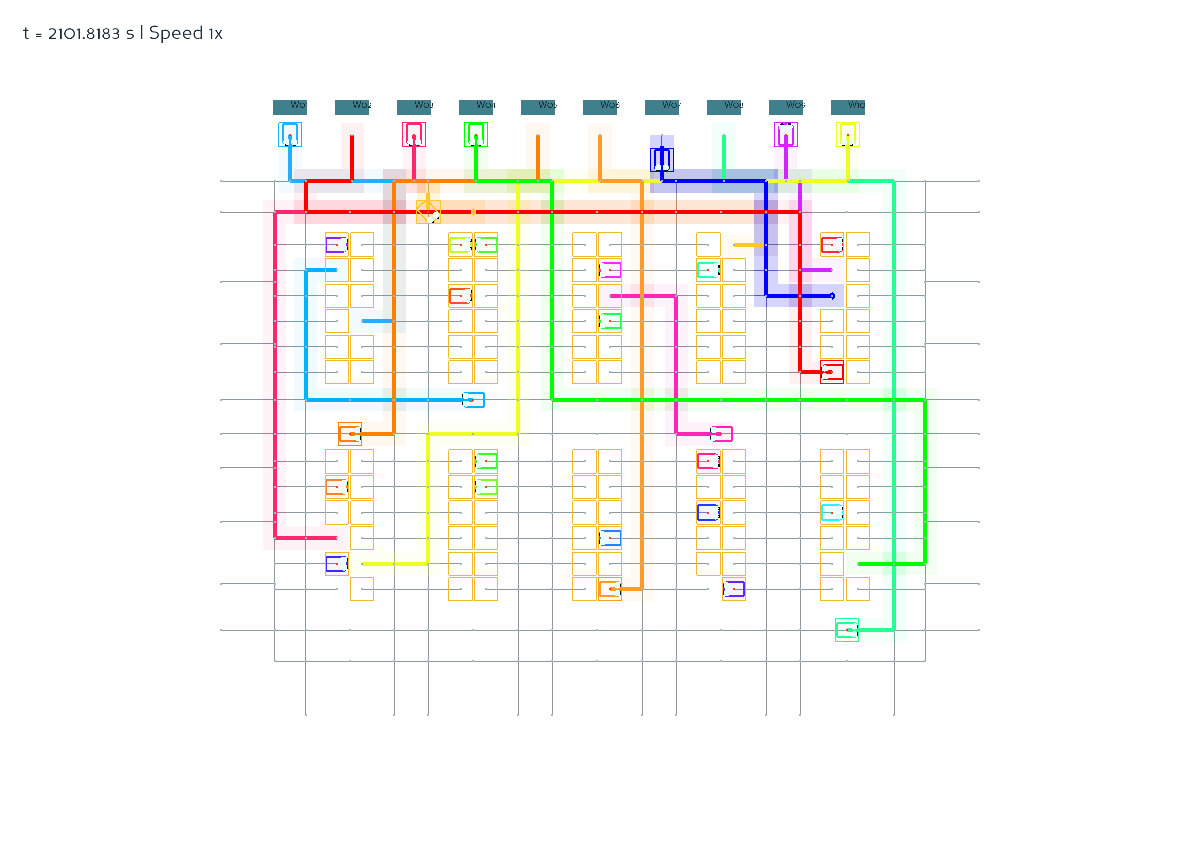
\includegraphics[width=.84\linewidth]{warehouse_top_A.png}\par
\smallskip
{\small (a) Alternative A (Forbidden, Forbidden). 50th shipment at 2,101.818~s. Full-run makespan 4,524.194~s and estimated fleet energy 1.920~kWh.}\par
\medskip
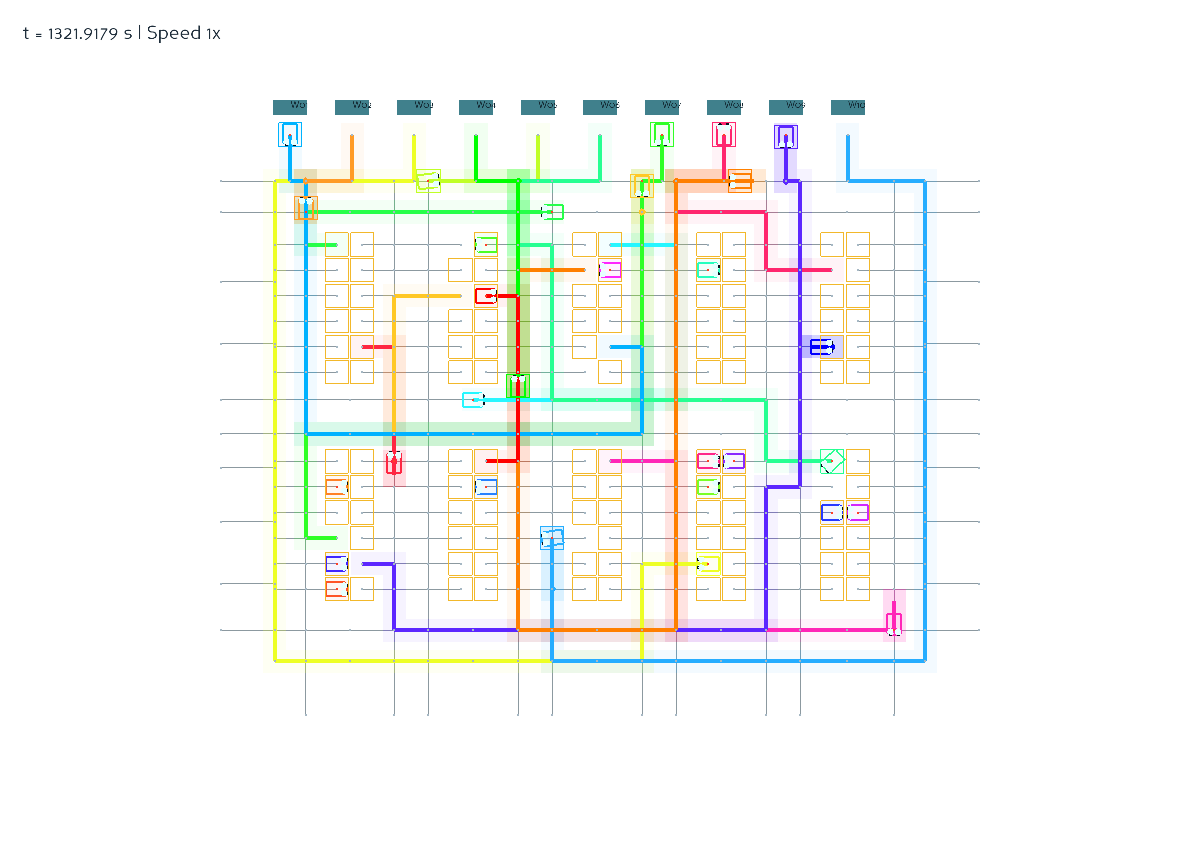
\includegraphics[width=.84\linewidth]{warehouse_top_D.png}\par
\smallskip
{\small (b) Alternative D (Allowed, Allowed). 50th shipment at 1,321.918~s. Full-run makespan 3,038.338~s and estimated fleet energy 1.579~kWh.}
\caption{Top views at the 50th shipment in the warehouse with 30 robots, 120 racks, and 10 inbound/outbound workstations.
Pale overlays show remaining path sweeps, and darker overlays show
remaining approved sweeps.}
\label{fig:warehouse-top}
\end{figure}
\clearpage
\section{Conclusion}
\begin{enumerate}
\item \textbf{Collision avoidance with remaining swept paths.}
The controller used sensor clearance reports to update the remaining
swept regions and checked their interference before authorizing motion.
The remaining approved sweep represents the space still covered by an
active movement approval and is checked against proposed movements
(Section~\ref{sec:remaining-movement-approval}).
All eight policy runs in the two controlled crossing layouts completed
with no detected collisions.

\item \textbf{Motion timing and energy estimation.}
The DEVS robot used acceleration, cruise, and braking profiles for
straight motion and rotation, with separate parameters for unloaded
and rack-carrying operation (Table~\ref{tab:motion-profiles}).
The profiles determined the timing of simulated motion. We estimated
battery energy from executed straight-motion profiles and auxiliary
power, including auxiliary draw during rotations. Lift and lower
completion events determined the load used in the warehouse energy
calculation.

\item \textbf{Two independently configurable intersection policies.}
We varied both policies in a $2\times2$ warehouse comparison.
\begin{enumerate}
\item \emph{Rolling passage.} A robot may receive permission to
continue while approaching an intersection. Under the stop-first
policy, it must stop before receiving permission to continue.
\item \emph{Stopping in intersection.} If permitted, an intersection
can serve as a temporary buffer. If forbidden, an approved movement
cannot end inside the intersection.
\end{enumerate}
In the single-crossing layout, an intersection stop delayed cross
traffic. In the two-crossing layout, the forward intersection served as a
buffer. With rolling passage allowed, the last robot in the upstream
queue cleared the crossing at 15.485~s with the buffer and 50.177~s
without it (Tables~\ref{tab:one-crossing-results}
and~\ref{tab:two-crossings-results}).

\item \textbf{Warehouse results.}
For 30 robots and 100 orders, alternative D achieved the lowest makespan and estimated fleet energy (Table~\ref{tab:warehouse-results}).
From A to D, makespan decreased by 32.8\% and estimated fleet
energy decreased by 17.8\%.
From A to C, makespan increased by 32.0\% and estimated fleet
energy increased by 28.5\%.
From B to D, makespan decreased by 32.9\% and estimated fleet
energy decreased by 19.7\%.
\end{enumerate}

The warehouse findings apply to the tested layout and order workload.
Dispatch timing and routes could vary with policy in the warehouse.
The energy values are simulation estimates for translational traction and
auxiliary power. Physical battery measurements and additional workloads
would test how well the reported savings transfer to other operating
conditions.

\clearpage
\appendix
\tikzset{
  devsphase/.style={draw, rounded corners=2pt, minimum height=7mm,
                    minimum width=20mm, align=center, font=\small\ttfamily},
  devsevent/.style={font=\scriptsize, align=center, fill=white, inner sep=2pt},
  devsarrow/.style={-{Stealth[length=2mm]}, semithick},
}
\section{RMFSController}
\label{app:rmfs-controller}
\texttt{RMFSController} is the atomic model that converts order and
execution events into robot commands. The phase is one component of
its state. \textbf{The \texttt{RoadMap} is another state component},
shared with and saved through the traffic manager. It holds each
robot's route, reported position, released progress, and
approved movement. The traffic manager uses this shared state to
check sweep interference and precedence. Two states in \texttt{Wait}
can therefore respond differently to the same passage request.
In the warehouse workflow,
the controller also tracks pending orders, rack and station
reservations, and service completion times.

In the \texttt{Command} phase the controller emits queued commands
with zero time advance. In \texttt{Wait} it reacts to incoming
reports or to the next scheduled service completion. Arrival and
clearance reports update occupancy and can make pending movements
eligible. A pre-braking request (Push) can trigger reconsideration
for its requesting robot. A clearance report (Pull) can trigger
reconsideration for robots waiting on the released space. If a
straight continuation is approved, the controller sends an
extension to the robot's active command.

\begin{figure}[H]
\centering
\begin{tikzpicture}
  \node[devsphase] (wait) at (0,0) {Wait};
  \node[devsphase] (cmd) at (7,0) {Command};
  \draw[devsarrow] (wait) to[bend left=22]
    node[devsevent,above]{Report yields a command\\or service timer expires} (cmd);
  \draw[devsarrow] (cmd) to[bend left=22]
    node[devsevent,below]{Emit queued commands; zero time advance} (wait);
  \draw[devsarrow] (wait) edge[loop left,min distance=8mm]
    node[devsevent,left]{Report yields\\no command} (wait);
  \draw[rounded corners=2pt] (-2.8,-1.55) rectangle (9.8,-5.12);
  \node[anchor=north west, font=\small\bfseries] at (-2.6,-1.68)
    {Controller state across phases};
  \node[anchor=north west, align=left, text width=5.25cm, font=\small]
    at (-2.6,-2.35) {
    \textbf{\texttt{RoadMap}}: routes and positions;\\
    release and approval progress.\\[3pt]
    Traffic: tasks and commands.\\[3pt]
    Warehouse: orders and timers.
  };
  \draw[gray!55] (3.05,-2.24) -- (3.05,-4.94);
  \node[font=\small\bfseries] at (6.37,-2.05) {RoadMap at an intersection};
  \fill[blue!18] (4.82,-3.86) rectangle (9.35,-3.22);
  \draw[gray!70] (7.43,-4.65) -- (7.43,-2.44);
  \draw[densely dashed, gray!80] (3.47,-3.54) -- (5.08,-3.54);
  \draw[blue!65!black, devsarrow] (5.08,-3.54) -- (9.03,-3.54);
  \draw[devsarrow, densely dashed] (7.43,-4.52) -- (7.43,-3.91);
  \draw[thin] (5.08,-3.78) -- (5.08,-4.18);
  \fill (5.08,-3.54) circle[radius=1.25pt];
  \node[devsevent,below] at (4.82,-4.19) {Release point};
  \node[devsevent] at (4.14,-3.07) {Released path};
  \node[devsevent] at (8.49,-3.01) {Remaining\\approved sweep};
  \draw[semithick, fill=white] (5.47,-3.79) rectangle (6.08,-3.29);
  \draw[thin] (5.78,-3.26) -- (5.78,-2.93);
  \node[devsevent,above] at (5.87,-2.92) {Reported robot\\position};
  \node[devsevent,anchor=west] at (7.58,-4.35) {Candidate\\movement};
\end{tikzpicture}
\caption{\texttt{RMFSController} phase transitions and selected internal
state. In the example, the candidate movement is held because its sweep
would intersect the remaining approved sweep. Incoming clearance reports
can update the \texttt{RoadMap} while the phase remains \texttt{Wait}.}
\label{fig:controller-phases}
\end{figure}

\section{MRobot}
\label{app:mrobot}
\texttt{MRobot} executes commands in physical time. Its state tracks
position, heading, the commanded path, the active profile, and
whether the rack is lifted. Aligned path segments are executed as
one straight run. The model uses \texttt{MoveTo} for translation
and \texttt{RotateTo} for in-place heading changes. Table%
~\ref{tab:motion-profiles} gives the translational and rotational
limits by load state. \texttt{LiftRack} and \texttt{LowerRack} are
timed phases that emit completion reports. In \texttt{Wait}, the
robot is stationary until a new command arrives.

The robot sends its active straight-motion plan to the paired
\texttt{PSensor} and reports arrivals and rotation boundaries to
the controller. When rolling passage is enabled, it can request an
extension before braking. An approved collinear extension of the
running profile preserves the executed prefix and starts the
replacement tail at the current speed. The robot sends the updated
plan to the sensor.

\begin{figure}[H]
\centering
\begin{tikzpicture}
  \node[devsphase] (wait) at (0,0) {Wait};
  \node[devsphase] (start) at (4.6,0) {StartMove};
  \node[devsphase] (move) at (9.2,0) {MoveTo};
  \node[devsphase] (lift) at (0,2.4) {LiftRack};
  \node[devsphase] (lower) at (3.5,2.4) {LowerRack};
  \node[devsphase] (turn) at (4.6,-2.65) {RotateTo};
  \node[devsphase] (collision) at (9.2,-4.3) {Collided};
  \node[font=\scriptsize] (any) at (4.6,-4.3) {Any operational phase};
  \draw[devsarrow] (wait) to[bend left=10]
    node[devsevent,above,pos=.60]{Move or orient command} (start);
  \draw[devsarrow] (start) to[bend left=10]
    node[devsevent,above]{Heading aligned; emit plan} (move);
  \draw[devsarrow,rounded corners=5pt] (move.north) -- (9.2,3.55)
    -- node[devsevent,above]{Final waypoint; report arrival} (-1.6,3.55)
    -- (-1.6,0) -- (wait.west);
  \draw[devsarrow] (wait) to[bend left=24] node[devsevent,left]{Lift} (lift);
  \draw[devsarrow] (lift) to[bend left=24] node[devsevent,right]{Lifted} (wait);
  \draw[devsarrow] (wait.north) to[out=65,in=195]
    node[devsevent,above,pos=.49]{Lower} (lower.west);
  \draw[devsarrow] (lower.south) to[out=230,in=63]
    node[devsevent,right,pos=.40]{Lowered} ([xshift=5mm]wait.north);
  \draw[devsarrow] (start) to[bend left=18] node[devsevent,right]{Entry turn} (turn);
  \draw[devsarrow] (turn) to[bend left=18] node[devsevent,left]{Turn done; resume path} (start);
  \draw[devsarrow] (move) --
    node[devsevent,sloped,below,pos=.44]{Turn at waypoint} (turn);
  \draw[devsarrow,rounded corners=5pt] (turn.west) --
    node[devsevent,below]{Orientation-only turn done} (0,-2.65) -- (wait.south);
  \draw[devsarrow] (move) edge[loop right,min distance=9mm]
    node[devsevent,right]{Straight waypoint\\or Push request} (move);
  \draw[devsarrow] (any) -- node[devsevent,above]{Collision} (collision);
\end{tikzpicture}
\caption{\texttt{MRobot} phase transitions. Motion extensions update
the command or active profile within the current phase.}
\label{fig:mrobot-phases}
\end{figure}

\section{PSensor}
\label{app:psensor}
\texttt{PSensor} is the atomic model for point clearance. Its input
motion plan gives the start time, origin, travel direction, footprint
half-sizes, monitored points, and executable motion profile. For
each monitored point, the model finds the distance along the run at
which the trailing footprint boundary clears the point. The inverse
motion profile converts that distance to a scheduled event time.
Endpoint occupancy is reported through the robot's arrival event.

The sensor waits in \texttt{Idle} for a plan and uses \texttt{Sensing}
to emit the clearances scheduled for its next event time. A
replacement plan reschedules pending clearances and preserves reports
already emitted for that run. The controller uses these reports to
advance released progress and reconsider movements.

\begin{figure}[H]
\centering
\begin{tikzpicture}
  \node[devsphase] (idle) at (0,0) {Idle};
  \node[devsphase] (sensing) at (6.5,0) {Sensing};
  \node[devsphase] (collision) at (3.25,-2.5) {Collided};
  \draw[devsarrow] (idle) to[bend left=21]
    node[devsevent,above]{Motion plan; schedule clearances} (sensing);
  \draw[devsarrow] (sensing) to[bend left=21]
    node[devsevent,below]{Emit last scheduled batch} (idle);
  \draw[devsarrow] (sensing) edge[loop right,min distance=9mm]
    node[devsevent,right]{Replacement plan; reschedule\\or emit batch; more events remain} (sensing);
  \draw[devsarrow] (idle) -- node[devsevent,below,sloped]{Collision} (collision);
  \draw[devsarrow] (sensing) -- node[devsevent,below,sloped]{Collision} (collision);
\end{tikzpicture}
\caption{\texttt{PSensor} phase transitions. In \texttt{Sensing}, the
next event time comes from the pending clearance schedule.}
\label{fig:psensor-phases}
\end{figure}

\begin{thebibliography}{99}
\bibitem{odonnell1989}
P. A. O'Donnell and T. Lozano-P\'erez.
Deadlock-free and collision-free coordination of two robot manipulators.
\emph{IEEE ICRA}, pp. 484--489, 1989.
\href{https://lis.csail.mit.edu/pubs/tlp/coordination-o-donnell.pdf}{Author-hosted PDF}.

\bibitem{hwang2026sweep}
M. H. Hwang.
\emph{A Sweep-Based Framework for Collision Avoidance among Mobile Robots}.
SOCS Project technical report, November 22, 2026.

\bibitem{hoenig2019}
W. H\"onig, S. Kiesel, A. Tinka, J. W. Durham, and N. Ayanian.
Persistent and robust execution of MAPF schedules in warehouses.
\emph{IEEE Robotics and Automation Letters}, 4(2):1125--1131, 2019.
\href{https://whoenig.github.io/publications/2019_RA-L_Hoenig.pdf}{Author manuscript}.

\bibitem{malikopoulos2018}
A. A. Malikopoulos, C. G. Cassandras, and Y. J. Zhang.
A decentralized energy-optimal control framework for connected automated
vehicles at signal-free intersections.
\emph{Automatica}, 93:244--256, 2018.
\href{https://doi.org/10.1016/j.automatica.2018.03.056}{DOI}.

\bibitem{pan2021}
X. Pan, B. Chen, L. Dai, S. Timotheou, and S. A. Evangelou.
Decentralized model predictive control for automated and connected electric
vehicles at signal-free intersections. \emph{IEEE CDC}, 2021.
\href{https://discovery.ucl.ac.uk/id/eprint/10131957/}{Accepted manuscript}.

\bibitem{verbeke2008}
W. Verbeke, C. M. J. Tamp\`ere, N. Van Paesschen, and B. Immers.
Modeling traffic operations on intersections using Monte-Carlo simulation
techniques. \emph{TRB 87th Annual Meeting}, paper 08-1585, 2008.
\href{https://www.mech.kuleuven.be/cib/verkeer/dwn/pub/PC2008B.pdf}{Institutional PDF}.

\bibitem{riazi2021}
S. Riazi, K. Bengtsson, and B. Lennartson.
Energy optimization of large-scale AGV systems.
\emph{IEEE Transactions on Automation Science and Engineering}, 18(2):638--649, 2021.
\href{https://doi.org/10.1109/TASE.2019.2963285}{DOI} and
\href{https://research.chalmers.se/en/publication/523467}{institutional record}.

\bibitem{malopolski2025}
W. Ma\l{}opolski, J. Zaj\k{a}c, W. Klein, and R. Cupek.
Impact of the deadlock handling method on the energy efficiency of a system
of multiple automated guided vehicles in a production environment described
as a square topology. \emph{Energies}, 18(23):6321, 2025.
\href{https://doi.org/10.3390/en18236321}{DOI}.

\bibitem{meissner2020}
M. Mei\ss ner and L. Massalski.
Modeling the electrical power and energy consumption of automated guided
vehicles to improve the energy efficiency of production systems.
\emph{International Journal of Advanced Manufacturing Technology}, 110:481--498, 2020.
\href{https://doi.org/10.1007/s00170-020-05796-8}{DOI}.

\bibitem{sperling2024}
M. Sperling and K. Furmans.
Energy requirement modeling for automated guided vehicles considering material
flow and layout data. \emph{Designs}, 8(3):48, 2024.
\href{https://doi.org/10.3390/designs8030048}{DOI}.

\bibitem{mir600}
Mobile Industrial Robots A/S.
\href{https://mobile-industrial-robots.com/it/prodotti/robot/mir600/specifiche}{MiR600 specifications}.
Manufacturer specification page, accessed November 23, 2026.

\bibitem{mir600datasheet}
Mobile Industrial Robots A/S.
\href{https://www.spie-escad.de/wp-content/uploads/MiR600-Specifications-2.96.pdf}{MiR600 Specifications}, p.~2, 2025.
Manufacturer data sheet hosted by SPIE ESCAD.
\end{thebibliography}

\end{document}
